\chapter{Calibração}

\section*{Célula de carga}
\begin{center}
    \begin{figure}[H]
    \centering
		
\includegraphics[scale=1.6]{Figuras/bateria/iconeimportante.png}
	    \label{iconeimportante}
    \end{figure} 
  
    	Informação importante sobre \textbf{CALIBRAÇÃO}
 \end{center}  

\par Dentre os sensores utilizados na base de lançamento e no foguete, apenas as células de cargas da balança são transdutores necessários de calibração, os demais sensores já possuem calibração de fábrica, onde geralmente seus coeficientes de calibragem ficam armazenados em ROM.

\par Para calibrar a balança, após a montagem com as duas células de carga 50 Kg e o módulo conversor HX711, será executado uma rotina de ajuste do sistema de medição em código C no microcontrolador ESP32 LoRa. De acordo com o Vocabulário Internacional de Metrologia Legal (VIML) o ajuste de um sistema de medição é conjunto de operações efetuadas num sistema de medição, de modo que ele forneça indicações prescritas correspondentes a determinados valores de uma grandeza a ser medida. 

\par Através do programa executado deve ser encontrado um valor aferido  denominado como Fator de Ajuste para  ser inserido no programa de medição da Balança com o conversor, e assim a calibração seja realizada.

\par O programa de ajuste fará uso da biblioteca \href{https://github.com/bogde/HX711}{HX711.h}, onde um objeto de peso conhecido deve ser lido pela balança, e a média dos valores retornados deve ser dividido pelo valor do peso real do objeto em KG, obtendo o fator de ajuste, que deve ser inserido como parâmetro da função “scale.set\textunderscore scale()” importada da biblioteca mencionada. Com esse fator de ajuste setado, obtém-se a calibração da balança, medindo então o do peso real do objeto.

\par A figura \ref{fig:Calibracao_balanca} apresenta o fluxograma do algoritmo de ajuste e calibração dos sensores da balança.

\begin{figure}[H]
  \centering
  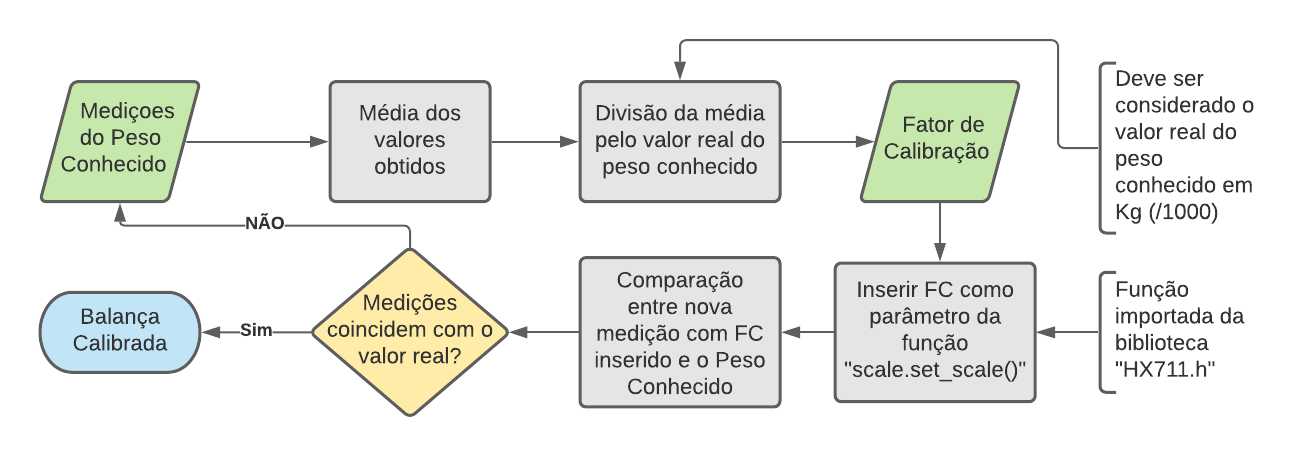
\includegraphics[width=\textwidth]{Figuras/Algoritmo de Calibração da Balança.png}
  \caption{Diagrama do algoritmo de calibração da balança } 
  {\footnotesize Fonte : Autor } 
  \label{fig:Calibracao_balanca}
\end{figure}
